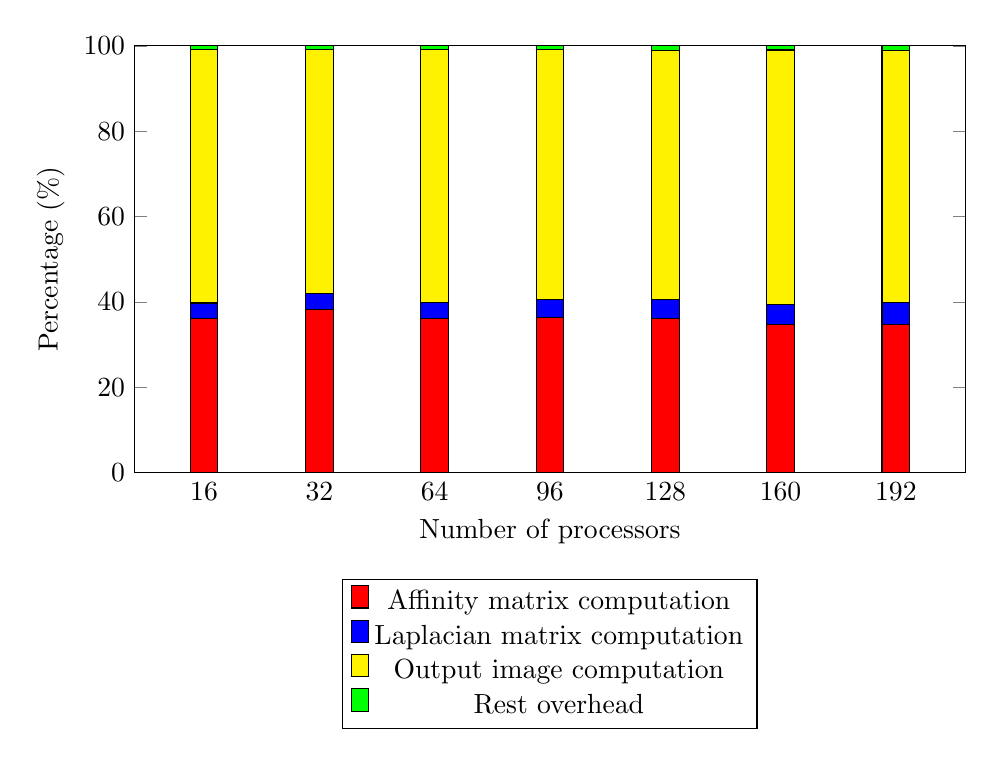
\begin{tikzpicture}
 \begin{axis}[
  ybar stacked,
  height=7cm,
  ymin=0,
  ymax=100,
  width=\textwidth,
  xlabel=Number of processors,
  symbolic x coords={
      16, 32, 64, 96, 128, 160, 192
  },
  xtick=data,
  legend style={
   at={(0.5, -0.25)},
   anchor=north
  },
  ylabel={Percentage (\%)}]
  \addplot[ybar, fill=red] plot coordinates {
   (16, 36.11)
   (32, 38.28)
   (64, 36.03)
   (96, 36.39)
   (128, 36.04)
   (160, 34.73)
   (192, 34.76)};
  \addplot[ybar, fill=blue] plot coordinates {
   (16, 3.62)
   (32, 3.59)
   (64, 3.90)
   (96, 4.19)
   (128, 4.49)
   (160, 4.71)
   (192, 5)};
  \addplot[ybar, fill=yellow] plot coordinates {
   (16, 59.49)
   (32, 57.32)
   (64, 59.18)
   (96, 58.52)
   (128, 58.47)
   (160, 59.57)
   (192, 59.21)};
  \addplot[ybar, fill=green] plot coordinates {
   (16, 0.78)
   (32, 0.81)
   (64, 0.89)
   (96, 0.9)
   (128, 1)
   (160, 1)
   (192, 1.03)};
  \legend{
   Affinity matrix computation,
   Laplacian matrix computation,
   Output image computation,
   Rest overhead}
 \end{axis}
\end{tikzpicture}
